% This is samplepaper.tex, a sample chapter demonstrating the
% LLNCS macro package for Springer Computer Science proceedings;
% Version 2.20 of 2017/10/04
%
\documentclass[runningheads]{llncs}
%
\usepackage{footnote}

\usepackage{graphicx}
\usepackage[british]{babel}
\usepackage[ruled,vlined]{algorithm2e}
\usepackage{lscape}
\usepackage{longtable}
\usepackage{tabularx}
\usepackage{booktabs}
\usepackage{xltabular}
\usepackage{array}
\usepackage{svg}
\usepackage{float} 
\usepackage{graphicx}
\graphicspath{ {./imgs/} }
\newcommand{\comment}[1]{}

\usepackage[ruled]{algorithm2e}

\BeforeBeginEnvironment{appendices}{\clearpage}

\newcommand{\algorithmfootnote}[2][\footnotesize]{%
  \let\old@algocf@finish\@algocf@finish% Store algorithm finish macro
  \def\@algocf@finish{\old@algocf@finish% Update finish macro to insert "footnote"
    \leavevmode\rlap{\begin{minipage}{\linewidth}
    #1#2
    \end{minipage}}%
  }%
}

% Used for displaying a sample figure. If possible, figure files should
% be included in EPS format.
%
% If you use the hyperref package, please uncomment the following line
% to display URLs in blue roman font according to Springer's eBook style:
% \renewcommand\UrlFont{\color{blue}\rmfamily}
\begin{document}
%
\title{Interoperable Machine Learning based Data Quality Evaluation in obstetrics real-world data}
%
%\titlerunning{Abbreviated paper title}
% If the paper title is too long for the running head, you can set
% an abbreviated paper title here
%
\author{João Coutinho-Almeida\inst{1,2}\orcidID{0000-0003-0882-6547} \and Carlos Saez \inst{}\orcidID{} \and
Ricardo João Cruz-Correia\inst{1,2}\orcidID{0000-0002-3764-5158} \and
Pedro Pereira Rodrigues,\inst{1,2}\orcidID{0000-0001-7867-6682} }
%
\authorrunning{J. Almeida et al.}
% First names are abbreviated in the running head.
% If there are more than two authors, 'et al.' is used.
%
\institute{ CINTESIS - Centre for Health Technologies and Services Research, University of Porto, Portugal \and
MEDCIDS – Faculty of Medicine of University of Porto, Portugal}
%
\maketitle              % typeset the header of the contribution
%
\begin{abstract}





\keywords{Data Quality \and Machine-learning \and Bayesian Networks \and Real-world data \and FHIR}
\end{abstract}
%
%Breast Cancer; personalised medicine; disease characteristics; machine learning; Cost-effectiveness; data warehousing; data integration
%
\section{Introduction}
With the wide spreading of healthcare information systems across all contexts of healthcare practice, the production of health-related data has followed this incremental behaviour. The potential for using this data to create new clinical knowledge and push medicine further is tempting \cite{martin-sanchezBigDataMedicine2014}.
However, to correctly use the data stored in Electronic Health Records (EHRs), the quality of the data must be robust enough to sustain the clinical decisions made based on this data. Data quality cannot be construed as a linear concept; it is intrinsically dependent on the context in which it is evaluated. The quality thresholds and dimensions required to classify the quality of the data depend on the purpose that we intend to use that very same data \cite{waljiElectronicHealthRecords2019}. These uses can be very distinct and have different impacts as well. For one, we can use data to support day-to-day decisions regarding individual patients' care \cite{verheijPossibleSourcesBias2018}. These decisions can include ones based on recorded information to understand a patient's history, clinical decision support systems based on this data, or even using the data to help support a more macro, public health-oriented decision. Another area is using information for management purposes. The data can be used by management bodies and regulatory authorities to extract metrics regarding the quality of care or reimbursement purposes. Thirdly, data can be used for research purposes, namely observational studies and, more recently, to support clinical trials through real-world evidence analysis \cite{coreyAssessingQualitySurgical2020,verheijPossibleSourcesBias2018,wengClinicalDataQuality2020}. 
So, all the EHR data-based decisions can only be as good as the data supporting them. Several studies have already warned about the lack of data quality in EHRs and how this can be a significant hurdle to an accurate representation of the population and potentially lead to erroneous healthcare decisions \cite{reimerDataQualityAssessment2016a,joukesImpactElectronicPaperBased2019a,huserMultisiteEvaluationData2016,zhangUnderstandingDetectingDefects2020,kramerImpactDataQuality2021,gigantiImpactDataQuality2019}.

There are several steps in the data lifecycle that can be prone to error, from data generation, where the data is registered by healthcare professionals, passing by data processing, whether inside healthcare institutions or by software engineers aiming to reuse data, to data interpretation and reuse, where investigators try to interpret the meaning of registered data \cite{wengClinicalDataQuality2020}.
So, with all of the data's possible uses added to the several steps that can introduce errors throughout the data lifecycle, data quality frameworks and sequential implementations can have very distinct approaches and methodologies to assess data quality. Data quality tools for checking data being registered live to support day-to-day decisions will be significantly different from one whose only purpose is to provide quality checks for research purposes. So, methodologies to tackle these issues are necessary for guaranteeing the quality of healthcare practice and the knowledge derived from EHR data. Consequently, in this paper, we propose:
\begin{itemize}
    \item Enlighten on the issues that can appear with a full deployment of such a tool;
    \item Suggestion of a creation of a single score for data quality for comparison of high-quality and low-quality records in a database.
    \item Assess how such a tool can work in early-stage real-world scenarios and how to work with obstetricians to improve data quality.
    \item Identify data quality issues on obstetrics data
\end{itemize}


%Data quality is a crucial aspect of the healthcare industry, as it impacts the accuracy of diagnoses, treatment plans, and patient outcomes. The reliability and accuracy of healthcare data have far-reaching consequences, including financial implications, patient safety, and legal ramifications. Inaccurate or incomplete data can lead to incorrect diagnoses, inappropriate treatments, and ultimately harm to patients. Therefore, ensuring the quality of healthcare data is essential to providing effective and safe healthcare services.

%One of the main reasons why data quality is so critical in healthcare is that healthcare data is often used to make important decisions, such as treatment plans, patient management, and resource allocation. Inaccurate or incomplete data can lead to misdiagnosis, inappropriate treatment, and increased healthcare costs. Furthermore, inaccurate data can hinder research efforts and impede the development of new treatments and therapies.

%Another key aspect of data quality in healthcare is its role in patient safety. Accurate and reliable data is essential for ensuring patient safety, particularly in areas such as medication management, clinical decision-making, and adverse event reporting. Poor data quality can lead to medication errors, adverse drug reactions, and other types of harm to patients.

%Finally, data quality is also important for legal and regulatory compliance in healthcare. Accurate and complete data is required for compliance with regulations such as HIPAA, the Affordable Care Act, and other regulatory requirements. Poor data quality can result in legal and financial penalties, as well as reputational damage for healthcare organizations.

%Overall, data quality is a crucial aspect of healthcare, with far-reaching implications for patient safety, healthcare costs, and regulatory compliance. Ensuring the quality of healthcare data requires a comprehensive approach that includes data governance, data management, data quality assurance, and ongoing monitoring and improvement efforts. By prioritizing data quality, healthcare organizations can provide better patient care, improve outcomes, and reduce costs.






\section{Background and Related Work}
%deve ser assim?os dois?ou separar?
There is already a significant number of papers trying to define data quality assessment frameworks for EHR data, all of them plausible and recommendable, already described in other papers \cite{bianAssessingPracticeData2020}. The literature has over 20 different methods, descriptions, and summaries of different frameworks over the years. Some may be highlighted from the review from Weiskopf et. al, \cite{weiskopfMethodsDimensionsElectronic2013}, where five data quality concepts were identified over 230 papers: Completeness, Correctness, Concordance, Plausibility, and Currency. 
Then Khan et al. tried to harmonize data quality assessment frameworks, which simplified all previous concepts into three main categories: Conformance, Completeness, and Plausibility, and two assessment contexts: Verification and Validation \cite{kahnHarmonizedDataQuality2016a}.
Then a review of Bian et al.  \cite{bianAssessingPracticeData2020} expanded on the previous ones, categorizing data quality into 14 dimensions and mapping them to the previous most known definitions. These were: currency, correctness, plausibility, completeness, concordance, comparability, conformance, flexibility, relevance, usability, security, information loss, consistency, and interpretability. 
Finally, the work of Saez et. al., defined a unified set of DQ dimensions: completeness, consistency, duplicity, correctness, timeliness, spatial stability, contextualization, predictive value and reliability \cite{saOrganizingDataQuality2012}.
Despite all of these comprehensive works, there is still no consensus regarding which one is best or which has taken the lead in usage. Moreover, looking at all of the descriptions related in the literature, a significant portion of concepts are overlapping, and sometimes hard to conceptualize such dimensions in practice. 

As for implementations, there are already some available, such as the work from \cite{phanAutomatedDataCleaning2020} where a tool created by primary care in the Flanders was built to assess completeness and percentage of values within the normal range.
The work from Liaw et al. \cite{liawQualityAssessmentRealworld2021} already reviewed some data quality assessment tools, like tools from OHDSI \cite{hripcsakObservationalHealthData2015} or TAQIH \cite{alvarezsanchezTAQIHToolTabular2019}. 
Additionally, we found some others with similar purposes and characteristics like the work presented data dataquieR \cite{schmidtFacilitatingHarmonizedData2021}, an R language-based package that can assess several data quality dimensions in observational health research data. 
Also, the work from Razzaghi et al. developed a methodology for assessing data quality in clinical data \cite{razzaghiDevelopingSystematicApproach2022}, taking into account the semantics of data and their meanings within their context. Furthermore, the work from Rajan et al. \cite{rajanContentAgnosticComputable2019} presented a tool that can assess data quality and characterize health data repositories. Parallel to this, Kaspner et al. created a tool called DQAStats that enables the profiling and quality assessment of the MIRACUM database, being possible to integrate into other databases as well \cite{kapsnerLinkingConsortiumWideData2021a}.


However, these tools are not meant to be used at the production level, assessing data as it is being registered or outputs reports for human consumption and not a quantitive metric for metric comparison. Furthermore, none of the non-agnostic tools were designed for obstetric EHR data nor had interoperability in mind. Finally, we have not seen, until the moment of this paper, any implementation that used machine learning to evaluate the correctness of the value.



\section{Materials}
The data was gathered from 9 different Portuguese hospitals regarding obstetric information: data from the mother, several data points about the fetus and delivery mode. The data is from 2019 to 2020. The software for collecting data was the same in every institution, and the columns were the same, even though the version of each software differed across hospitals. Across the different hospitals, data rows ranged from 2364 to 18177. The sum of all rows is 73351 rows. The data dictionary is in appendix \ref{appendix:data_dict}.

For this purpose, we took the Khan harmonized framework since we understood it as simpler to communicate we feel that the three main categories are indeed non-reducible, which makes sense from an organizational standpoint. Furthermore, the work done by Khan et al. with mapping to already existing frameworks could help compare this work with others who felt the need to use other frameworks.
With this in mind, we will use three main categories, Completeness, Conformance and Plausibility. Completeness relates to missing data. Conformance relates to the compliance of the data representation, like formatting, computational conformance and other data standards implemented. Plausibility relates to how believable the values are.

%TC:ignore
\begin{figure}[htbp]
\centering
\caption{Dimensions of data quality}\label{fig:categories} 
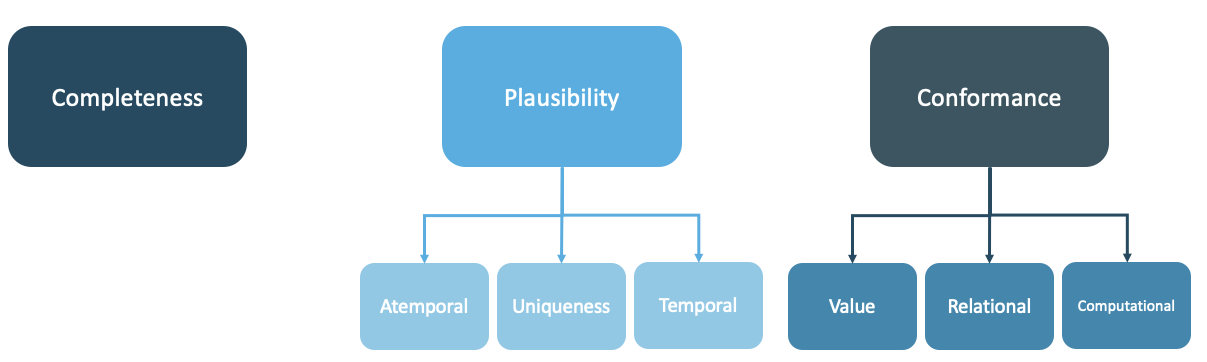
\includegraphics[scale=0.29]{imgs/data-quality-v1.png}
\end{figure}
%TC:endignoregrama

\section{Methods}
We wrote all of the code in Python 3.10.6 with the usage of the scikit-learn library for preprocessing, and evaluation \cite{scikit-learn}. 
For plausibility, a Bayesian network was used. We used this model due to the possiblity of using a single model for classifying the plausibility of all columns and due to its interpretable nature.
The networks was created with the pgmpy package \cite{pgmpy}. For creating the network, all null representations were standardized. Data was prepossessed with the removal of features with high missing rates ($>$ 80\% overall). All missing value representations were standardized. The imputation process was performed with the median for continuous and a new category (NULLIMP) for categorical variables. Then, the continuous variables were discretized into three bins defined by quantile. The evaluation was done with cross-validation with 10 splits and two repetitions for each column as the target. 

As for  Z-Scores, they were defined for all continuous variables based on the interquartile range. Then, rows were also assessed with distance analysis, with Local Outlier Factor and Elliptic Envelope from scikit-learn and the outlier-tree algorithm. We also added a rule engine, using the \textit{great\_expectations} package. Rules were defined by the team, focusing on impossible numbers present in age, weight, or relationship between variables. As for missing information was created with all the data, creating the scoring based on the inverse of the missing percentage. Missing detection was based on primary key variables. For completeness, we used the inverse of the percentage of nulls in the training set.
The API for serving the prediction models was developed with FastAPI. So, the methods applied in terms of the DQA framework shown in figure \ref{fig:categories} are described in the table \ref{tab:methods}.

\begin{table}[htpb]
\caption{Implemented Methods} \label{tab:methods}
\renewcommand{\arraystretch}{1.4}
\setlength{\tabcolsep}{10pt}

\begin{tabularx}{\textwidth}{ p{2cm} p{3.5cm} X }
\hline
 Category   & Subcategory           & Method   \\ \hline
Completeness     & N/A               & Score by the inverse percentage of missing in the train data         \\ 
Plausibility & Atemporal Plausibility & Bayesian model prediction based on the other values of row \\ 
Plausibility & Atemporal Plausibility         & Z-score for column value based on IQR train data       \\    
Plausibility & Atemporal Plausibility           & Elliptic Envelope                       \\ 
Plausibility & Atemporal Plausibility           & Local Outlier Factor                \\ 
Conformance & Value Conformance           & Manual Rule engine                           \\ 
Plausibility & Atemporal Plausibility           & Manual Rule engine                      \\ 
Plausibility & Atemporal Plausibility           & outlier-tree                      \\ 
\hline
\end{tabularx}

\end{table}
The method of scoring was to obtain a single value that could grasp the quality of the row or patient.
To assess the tool's usefulness, we will implement it in a production environment and collect metrics regarding the data being produced. Then we intended to present some results to selected obstetrics clinicians for them to assess how likely the information is to be suitable for usage. We will also compare the results with the ones from the model to make sanity checks regarding the model's performance and adequacy. We aim to use Kendal Tau and Average Spearman's Rank Correlation Coefficient. Kendall Tau is a non-parametric statistic used to measure the strength and direction of the association between two ordinal variables. It calculates the difference between the number of concordant and discordant pairs of observations, normalized to ensure a value between -1 (perfect disagreement) and 1 (perfect agreement). Spearman's rank correlation coefficient is a non-parametric measure that assesses the strength and direction of a monotonic relationship between two ranked variables. It is based on the ranked values of the variables rather than their raw data, producing a value between -1 (perfect inverse relationship) and 1 (perfect direct relationship).


\section{Results}
A Bayesian network with structure and parameters learned from the training dataset reached an average of Area Under the Receiver Operating Characteristic Curve of 0.857. The results are in the table \ref{tab:result_auc}.



\begin{table}[htpb]
 \caption{Validation Results: Column acronym with AUROC along with 95\% CI} \label{tab:result_auc} 

\renewcommand{\arraystretch}{1.2}
%\setlength{\tabcolsep}{8pt}
\centering
\begin{tabular} { p{1.5cm} p{1.5cm} p{3cm} p{1.5cm} p{1.5cm} l }
\hline
AP & 0.944 & [0.943, 0.945] & VNH & 0.894 & [0.893, 0.895] \\
AG & 0.797 & [0.778, 0.816] & TPEE & 0.816 & [0.815, 0.816] \\
EA & 0.969 & [0.968, 0.969] & AA & 0.751 & [0.743, 0.758] \\
CA & 0.958 & [0.958, 0.958] & GR & 0.931 & [0.93, 0.932] \\
IA & 0.638 & [0.637, 0.638] & V & 0.983 & [0.982, 0.983] \\
PI & 0.881 & [0.88, 0.881] & TP & 0.866 & [0.865, 0.868] \\
IMC & 0.881 & [0.881, 0.882] & VCS & 0.79 & [0.789, 0.791] \\
NRC & 0.75 & [0.75, 0.75] & ANP & 0.942 & [0.938, 0.946] \\
IGA & 0.968 & [0.968, 0.969] & GS & 0.514 & [0.507, 0.52] \\
SGP & 0.974 & [0.974, 0.974] & S & 0.896 & [0.896, 0.897] \\
VA & 0.974 & [0.974, 0.974] & VP & 0.771 & [0.77, 0.772] \\
TG & 0.728 & [0.726, 0.73] & TPNP & 0.952 & [0.951, 0.952] \\
\hline
 \multicolumn{6}{c}{\textbf{Average}  \textbf{0.857 [0.846, 0.868]}} \\

\hline
\end{tabular}
\end{table}


The network is as represented in figure \ref{fig:network}.
%TC:ignore
\begin{figure}[htbp]
\centering
\caption{Network learned}\label{fig:network} 
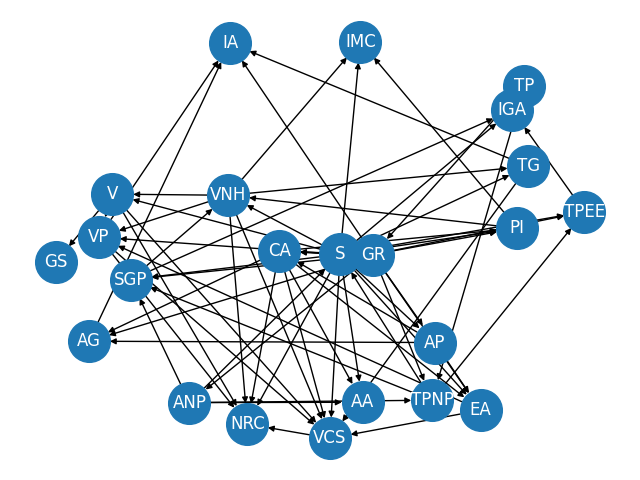
\includegraphics[scale=0.68]{imgs/network.png}
\end{figure}
%TC:endignore

As for the rules created, they were conformance based, like the format of dates, and conformance to the value set (i.e. Robson group, bishop scores, or delivery types). We also added plausibility rules, like expected values for BMI, weight and gestational age. We also added plausibility for the relationship between columns, namely weight across different weeks of gestation. We have also added a relationship of greatness between ecography weights more than 5 weeks apart. 





\subsection{Deployment \& Validation}
The purpose of this model is to be served as an API for usage within a healthcare institution and act as a supplementary decision support tool for obstetrics teams. Although a concrete, vendor-specific information model and health information system were initially used, our goal is to develop a more universal clinical decision support system. This system should be usable across all systems involved in birth and obstetrics departments. Therefore, we constructed it using the Health Level 7 (HL7) Fast Healthcare Interoperable Resources (FHIR) R5 version standard. This approach simplifies the process of API interaction.
Rather than utilizing a proprietary model for the data, we based our decision on the use of FHIR resources: Bundle and Observation. These resources handle the request and response through a customized operation named "\$quality\_check". Our intention is to publish the profiles of these objects to streamline API access via standardized mechanisms and data models. The current version of the profiles can be accessed at this URL: \url{https://joofio.github.io/obs-cdss-fhir/}. 


For validation, we deployed the tool in docker format in a hospital to gather new data. We gathered 3231 new cases and returned a score for quality as exemplified in figure \ref{fig:scores}. Being that the score is from 0 to 1, the average score was 0.23 and IQR was 0.03. We also used the clinician from one of the hospitals that we get data from and asked this clinician to assess 10 records in terms of quality. We gathered the 10 records at random and asked the clinician to assess them in terms of quality. Our purpose was then to compare the rankings of each evaluator; the model and the clinician, in order to assess how similar they were as can be seen in figure \ref{fig:clinical}.





%TC:ignore
\begin{figure}[htbp]
\centering
\caption{Model score for newly seen data}\label{fig:scores} 
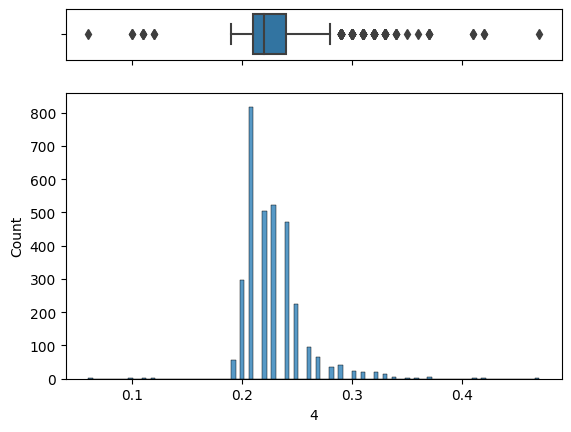
\includegraphics[scale=0.78]{imgs/Scoring.png}
\end{figure}
%TC:endignore

%TC:ignore
\begin{figure}[htbp]
\centering
\caption{Comparasion of clinical assessment of records with the model}\label{fig:clinical} 
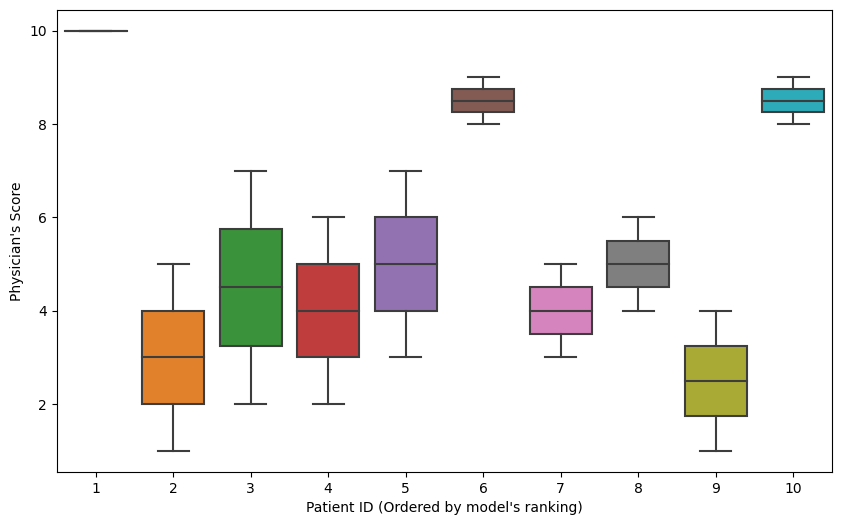
\includegraphics[scale=0.52]{imgs/clinical_assessment.png}
\end{figure}
%TC:endignore

\section{Discussion}
The first thing to address is that data quality is still an elusive concept since it has a contextual dimension and the quality of the record depends on the usage of the information. For example, data aimed at primary usage and day-to-day healthcare decisions about a patient will have different requirements regarding the importance of some variable or completeness of information very different from data needed to create summary statistics for key performance indicators extraction. 
Moreover, the data is still very vendor-specific. Even though we used an interoperability standard, the semantic layer, more connected with terminology is still lacking. This is an issue to be addressed in order to improve the interoperability of the standard. Moreover, we do not know how the training done with this data is generalizable to other vendors. One opportunity arises of mapping all of this data to a widely used terminology like SNOMED CT or LOINC. Nevertheless, the usage of FHIR and the fact that the data is mapped to a standard terminology, makes it easier to use the data in other systems and to compare the results with other studies. Furthermore, being available freely and online makes it easier to understand how to map vendor-specific datasets to the model and use it in other contexts.
Regarding the model, the usage of explainable methodologies like outlier-tree and transparent models like Bayesian networks are vital for clinical application. Since we use a single model to classify possible errors in the records, the ability to try to show clinicians why that value was tagged is of uttermost importance in order to get feedback and action from humans. From the experience gathered with the study, we believe that a weaker but transparent model could have more impact than better performant but opaque ones. If explainability and interpretability are important for any ML problem, this need only increases when we are dealing with such subjective concepts as data quality.



Regarding the clinical evaluation, we found out that asking clinicians to purely assess the quality of a record in an ehr is not an easy task. We found out that for a proper assessment, a context and objective must be defined in order to make the evaluation more objective. Moreover, the ranking methodology, even though is very useful for comparing with the model, it is not easy for clinicians to order 10 records when some of them have the "same level" of quality. This is a very important aspect to take into account when designing the evaluation of data quality. Probably a categorical evaluation of yes/no could be more useful and then compare with the ordering of the model and define thresholds based on that. These reasons are probably the cause behind the great variability between clinicians and between clinicians and the model. However, we do see a tendency for a higher agreement of the worst quality results than the best ones. 
This result suggests that the system may not be suitable for ranking good-quality records and clinicians are also not able. However, it could be useful to alert for low-quality ones, which is also a very important task with a great impact on the quality of the data. These findings are supported not only by \ref*{fig:clinical} but also by figure \ref*{fig:scores} where we can add some threshold for the need for a human review. From the preliminary data in the questionnaires and looking at the graph, we believe that a threshold of around 0.3 could be a good starting point. However, this is a very subjective decision, and it should take into account the context and the objective of the evaluation. For example, if the objective is to use the data for research, a higher threshold could be used. On the other hand, if the objective is to use the data for day-to-day clinical decisions, a lower threshold could be used.


For the next steps, we believe a research path could be of identifying contexts for applying data quality checks like primary usage, research purposes, and aggregated analysis for decision-making among others could help better target those contexts and the importance of each variable for those use cases. This could be interesting to add to the tool in order to weigh the different variables according to the context. 

%discutir que dependendendo da pessoa /context/profissao/objecti pode ser preciso dar pesos diferentes a diferentes colunas.
%para dar GDH nao ha coisas que sao precisas mas ha coisas vitais
%para financeiro ha so umas precisas (tipo meds e procs)
%para clinico ha outras e por ai fora

\section{Conclusion}
This work is still an early draft of a production-ready tool. However, we feel the work done is already a valuable insight into how to use data quality frameworks and several statistical tools in order to assess ehr data quality. This is a fundamental process not only to guarantee the quality of data for primary usage on a day-to-day but also for securing quality for secondary analysis and usage.
We believe the fact that we created an interoperable tool that was trained on real obstetrics data from 9 different hospitals and has the ability to provide a single score for a clinical record can help institutions, academics, and ehr vendors implement data quality assessment tools in their own systems and institutions.

For the next steps, we would like to further evaluate the score and its relationship with clinical usefulness. This would also include a further assessment of a  threshold for the score for defining a record that would require human attention.

%
% ---- Bibliography ----
%
% BibTeX users should specify bibliography style 'splncs04'.
% References will then be sorted and formatted in the correct style.
%
% \bibliographystyle{splncs04}
% \bibliography{mybibliography}
%
%\begin{thebibliography}{8}
%\bibliographystyle{splncs04}
\bibliographystyle{unsrt}

\bibliography{bibliography}
%\end{thebibliography}
\appendix

\section{Data Dictionary}
\label{appendix:data_dict}
\begin{table}[H]
\begin{tabularx}{\textwidth}{| l  | X |}
\toprule
Initial  &    Description \\
\midrule
IA &  Mother Age \\
GS  & Blood Group \\
PI &   Weight at the beginning of pregnancy \\
PAI &  Weight on Admission \\
IMC &   BMI \\
CIG &   If Smoker During Pregnancy \\
APARA  & Number of previously born babies\\
AGESTA  &   Number of Pregnancies   \\
EA &     Number of Previous Eutocic Deliveries with no assistance \\
VA &      Number of Previous Eutocic Deliveries with help of vacuum extraction \\
FA &     Number of Previous Eutocic Deliveries with help of forceps \\
CA &   Number of  Previous C-sections \\
TG &     Pregnancy Type (spontaneous, In vitro fertilisation...) \\
V &     If the pregnancy was accompanied by physician \\
NRCPN &     Number of prenatal consultations \\
VH &      If the pregnancy was accompanied by a physician in a hospital \\
VP &    If the pregnancy was accompanied by a physician in a private clinic \\
VCS &  If the pregnancy was accompanied by a physician in a primary care facility \\
VNH &    If the pregnancy was accompanied by a physician in the hospital the delivery was made \\
B  & Pelvis Adequacy \\
AA & Baby's Position on Admission \\
BS &  Bishop Score \\
BC &   Bishop Score Cervical Consistency\\
BDE &  Bishop Score Fetal Station \\
BDI &  Bishop Score Dilatation \\
BE  &   Bishop Score Effacement \\
BP & Bishop Score Cervical Position \\
IGA  & Number of Weeks on Admission \\
TPEE  & If the delivery was spontaneous   \\
TPEI  &  If the delivery was induced  \\
RPM  & If there was a rupture of the amniotic pocket before delivery began \\
DG &  Gestational Diabetes \\
TP & Delivery Type \\
ANP  & Baby's Position on Delivery \\
TPNP  & Actual Type of Delivery\\
SGP  & Pregnancy Weeks on Delivery \\
GR  &   Robson Group \\
\bottomrule
\end{tabularx}
\end{table}




\end{document}
